\newsec{Caratterizzazione dell'elettromagnete}{Studio dell'uniformità del campo magnetico dentro al traferro, \\ e del ciclo di isteresi del magnete.}

Prima di studiare l'effetto Hall, abbiamo caratterizzato l'elettromagnete in modo da poter misurare indirettamente il campo magnetico usando la corrente di alimentazione.

\subsection{Uniformità del campo magnetico}

Abbiamo cominciato valutando l'intensità del campo magnetico in vari punti del traferro: suddividendolo in intervalli regolari abbiamo riportato i valori misurati con un magnetometro (\ldots) su un istogramma.
Si riconosce una regione di uniformità al centro del traferro (in \cref{fig:uniform-magnet}) in cui gli effetti di bordo sono trascurabili: è proprio qui che abbiamo sempre posizionato la sonda di Hall.

In particolare, prendiamo la semidifferenza tra i valori di $ B $ misurati in questa regione:
\begin{equation}
\Delta B = (\ldots \pm \ldots) \unit{mT}
\end{equation}
come il limite minimo sull'incertezza del campo magnetico.

\subsection{Ciclo di isteresi}

Per valutare la risposta del magnete alla corrente di alimentazione delle bobine nella regione di uniformità (punto centrale del traferro), abbiamo caratterizzato il ciclo di isteresi del magnete.
Percorrendo interamente due cicli arrivando fino alla saturazione, abbiamo raccolto i dati in \cref{tab:hysteresis}, e in \cref{fig:hysteresis}.

\begin{table}
\centering \small
\begin{tabular}{cccccccc}
$B_\text{down,1}$ & $\delta B_\text{down,1}$ & $i_\text{down,1}$ & $\delta i_\text{down,1}$ & $B_\text{up,1}$ & $\delta B_\text{up,1}$ & $i_\text{up,1}$ & $\delta i_\text{up,1}$ \\
\hline
355.200 & 18.760 & 1.602 & 0.034 & -358.100 & 18.905 & -1.605 & 0.034 \\
322.500 & 17.125 & 1.406 & 0.031 & -322.400 & 17.120 & -1.400 & 0.031 \\
279.300 & 14.965 & 1.180 & 0.028 & -282.900 & 15.145 & -1.195 & 0.028 \\
243.000 & 13.150 & 0.999 & 0.025 & -244.400 & 13.220 & -1.007 & 0.025 \\
200.400 & 11.020 & 0.800 & 0.022 & -201.600 & 11.080 & -0.806 & 0.022 \\
159.000 & 8.950 & 0.619 & 0.019 & -154.400 & 8.720 & -0.599 & 0.019 \\
104.500 & 6.225 & 0.393 & 0.002 & -94.700 & 5.735 & -0.353 & 0.002 \\
59.800 & 3.990 & 0.208 & 0.001 & -58.900 & 3.945 & -0.206 & 0.001 \\
9.300 & 1.625 & 0.000 & 0.000 & -8.700 & 1.625 & 0.000 & 0.000 \\
-47.700 & 3.385 & -0.234 & 0.001 & 40.200 & 3.010 & 0.202 & 0.001 \\
-87.700 & 5.385 & -0.400 & 0.016 & 89.600 & 5.480 & 0.405 & 0.016 \\
-136.400 & 7.820 & -0.603 & 0.019 & 138.900 & 7.945 & 0.611 & 0.019 \\
-183.300 & 10.165 & -0.802 & 0.022 & 189.100 & 10.455 & 0.825 & 0.022 \\
-228.500 & 12.425 & -1.011 & 0.025 & 231.900 & 12.595 & 1.025 & 0.025 \\
-269.900 & 14.495 & -1.201 & 0.028 & 268.800 & 14.440 & 1.198 & 0.028 \\
-314.100 & 16.705 & -1.419 & 0.031 & 310.600 & 16.530 & 1.403 & 0.031 \\
-349.400 & 18.470 & -1.604 & 0.034 & 350.700 & 18.535 & 1.615 & 0.034 \\
-383.800 & 20.190 & -1.805 & 0.037 & 381.700 & 20.085 & 1.798 & 0.037 \\
&&&&&&&\\
$B_\text{down,2}$ & $\delta B_\text{down,2}$ & $i_\text{down,2}$ & $\delta i_\text{down,2}$ & $B_\text{up,2}$ & $\delta B_\text{up,2}$ & $i_\text{up,2}$ & $\delta i_\text{up,2}$ \\
\hline
356.300 & 18.815 & 1.599 & 0.034 & -358.700 & 18.935 & -1.610 & 0.034 \\
319.600 & 16.980 & 1.383 & 0.031 & -325.100 & 17.255 & -1.409 & 0.031 \\
281.700 & 15.085 & 1.192 & 0.028 & -284.800 & 15.240 & -1.201 & 0.028 \\
243.800 & 13.190 & 1.003 & 0.025 & -240.800 & 13.040 & -0.987 & 0.025 \\
198.000 & 10.900 & 0.788 & 0.022 & -202.500 & 11.125 & -0.808 & 0.022 \\
157.700 & 8.885 & 0.611 & 0.019 & -156.000 & 8.800 & -0.603 & 0.019 \\
108.300 & 6.415 & 0.409 & 0.016 & -106.200 & 6.310 & -0.399 & 0.002 \\
56.700 & 3.835 & 0.197 & 0.001 & -56.400 & 3.820 & -0.195 & 0.001 \\
8.900 & 1.625 & 0.000 & 0.000 & -8.700 & 1.625 & 0.000 & 0.000 \\
-44.500 & 3.225 & -0.219 & 0.001 & 42.500 & 3.125 & 0.210 & 0.001 \\
-88.400 & 5.420 & -0.400 & 0.016 & 87.200 & 5.360 & 0.395 & 0.002 \\
-141.800 & 8.090 & -0.621 & 0.019 & 137.500 & 7.875 & 0.602 & 0.019 \\
-185.500 & 10.275 & -0.808 & 0.022 & 190.200 & 10.510 & 0.830 & 0.022 \\
-227.300 & 12.365 & -1.001 & 0.025 & 227.700 & 12.385 & 1.000 & 0.025 \\
-272.300 & 14.615 & -1.213 & 0.028 & 272.700 & 14.635 & 1.208 & 0.028 \\
-313.600 & 16.680 & -1.416 & 0.031 & 321.900 & 17.095 & 1.456 & 0.032 \\
-349.900 & 18.495 & -1.606 & 0.034 & 349.500 & 18.475 & 1.602 & 0.034 \\
-383.800 & 20.190 & -1.807 & 0.037 & 381.700 & 20.085 & 1.798 & 0.037 \\
- & - & - & - & 414.900 & 21.745 & 2.013 & 0.040 \\
- & - & - & - & 452.000 & 23.600 & 2.318 & 0.045 \\
- & - & - & - & 476.700 & 24.835 & 2.627 & 0.049 \\
- & - & - & - & 495.400 & 25.770 & 2.900 & 0.053 \\
- & - & - & - & 499.900 & 25.995 & 2.977 & 0.055 
\end{tabular}
\caption{Dati relativi ai cicli di isteresi}
\label{tab:hysteresis}
\end{table}

\begin{figure}
\centering
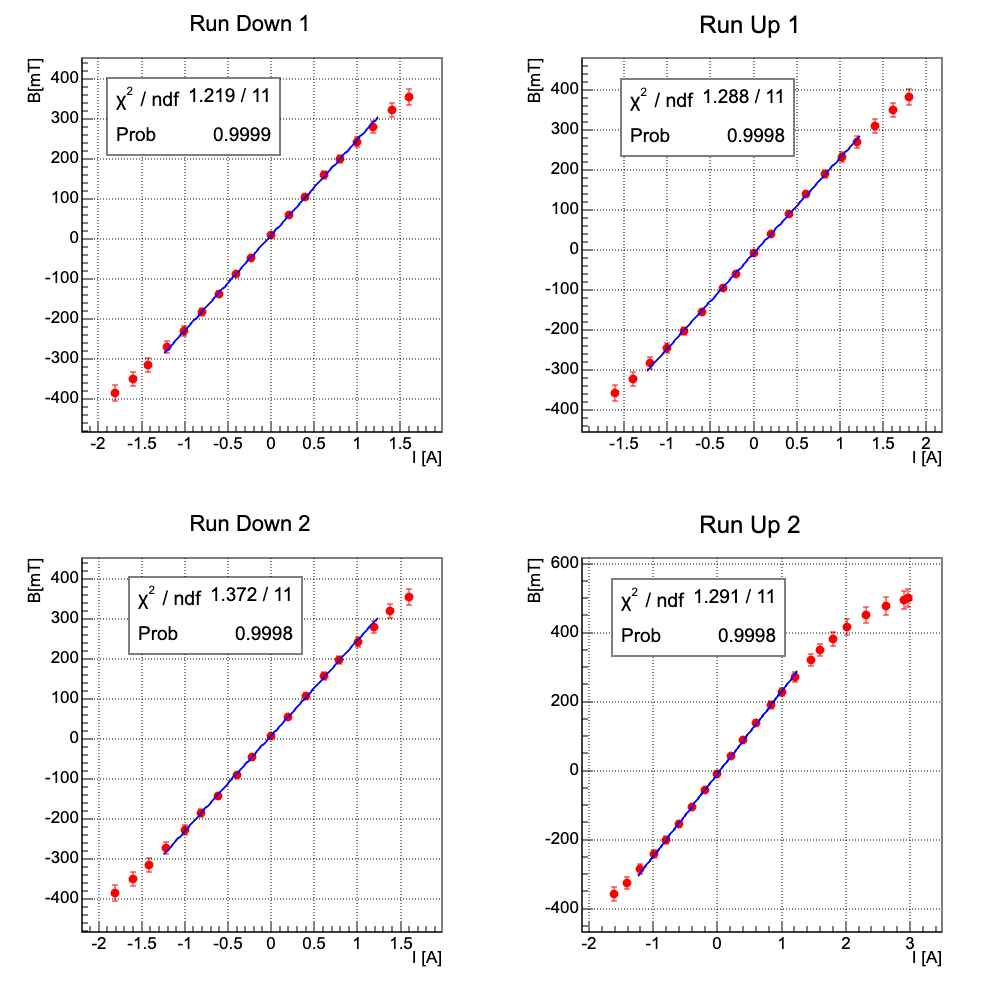
\includegraphics[width=0.84 \textwidth]{./figs/hysteresis.png}
\caption{ciao}
\label{fig:hysteresis}
\end{figure}


Il magnete si comporta come un materiale molle: la forza coercitiva appare debole.
Si osserva un'area compresa tra ciclo in discesa e salita estremamente ridotta rispetto ai cicli di isteresi di materiali duri. 

Nello specifico, abbiamo effettuato delle regressioni lineari nelle regioni di linearità dei cicli di isteresi, ricavando le stime degli andamenti del campo magnetico $ B $ con la corrente di alimentazione nelle bobine $ I $:
\begin{align}
B_\text{up,1} &= (\ldots \pm \ldots) \unit{mT} + (\ldots \pm \ldots) \unit{mT / A} \cdot I \\
B_\text{down,1} &= (\ldots \pm \ldots) \unit{mT} + (\ldots \pm \ldots) \unit{mT / A} \cdot I \\
B_\text{up,2} &= (\ldots \pm \ldots) \unit{mT} + (\ldots \pm \ldots) \unit{mT / A} \cdot I \\
B_\text{down,2} &= (\ldots \pm \ldots) \unit{mT} + (\ldots \pm \ldots) \unit{mT / A} \cdot I.
\end{align}

In particolare, possiamo verificare la compatibilità tra le quote delle coppie di salita e di discesa (con $ Z_\text{up} = \ldots $ e $ Z_\text{down} = \ldots $, accettati al $ 5 \% $), e pure quella tra tutti i coefficienti angolari (con \ldots). \help{maybe insert into a table?}

In virtù di questo, abbiamo calcolato gli andamenti medi (pesati per gli errori) sui cicli in salita/discesa, e su un ciclo generico:
\begin{align} \label{eq:hysteresis-up}
B_\text{up} &= (\ldots \pm \ldots) \unit{mT} + (\ldots \pm \ldots) \unit{mT / A} \cdot I \\ \label{eq:hysteresis-down}
B_\text{down} &= (\ldots \pm \ldots) \unit{mT} + (\ldots \pm \ldots) \unit{mT / A} \cdot I \\ \label{eq:hysteresis-mean}
B_\text{mean} &= (\ldots \pm \ldots) \unit{mT} + (\ldots \pm \ldots) \unit{mT / A} \cdot I
\end{align}
dove l'errore sulla quota di $ B_\text{mean} $ lo abbiamo stimato con la differenza tra le quote di $ B_\text{up} $ e $ B_\text{down} $.
